\section{1174039 - Liyana Majdah Rahma}

\subsection{Teori}
\begin{enumerate}
\begin{itemize}

        \item Jelaskan dengan ilustrasi gambar sendiri apa perbedaan antara vanilla GAN dan cGAN.

Vanilla GAN Vanilla GAN adalah tipe GAN paling sederhana. Di sini, Generator dan Diskriminator adalah perceptron multi-layer sederhana. Dalam vanilla GAN, algoritma ini sangat sederhana, ia mencoba untuk mengoptimalkan persamaan matematika menggunakan keturunan gradien stokastik.CGAN (Conditional GAN), label bertindak sebagai ekstensi ke ruang laten z untuk menghasilkan dan membedakan gambar dengan lebih baik. 

	\begin{figure}[H]
            	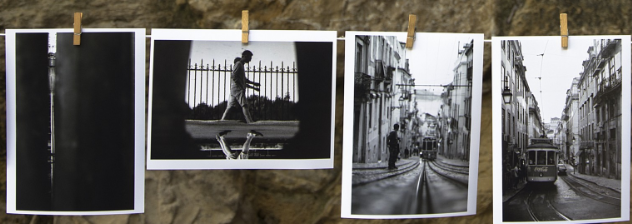
\includegraphics[width=4cm]{figures/1174039/chapter9/teori1.PNG}
           	\centering
           	\caption{Valina GAN-cGAN}
        	\end{figure}

        \item Jelaskan dengan ilustrasi gambar sendiri arsitektur dari Age-cGAN.

Age cGAN ialah dengan mengkondisikan model pada informasi tambahan dimungkinkan untuk mengarahkan proses pembuatan data. Pengkondisian semacam itu dapat didasarkan pada label kelas.

	\begin{figure}[H]
		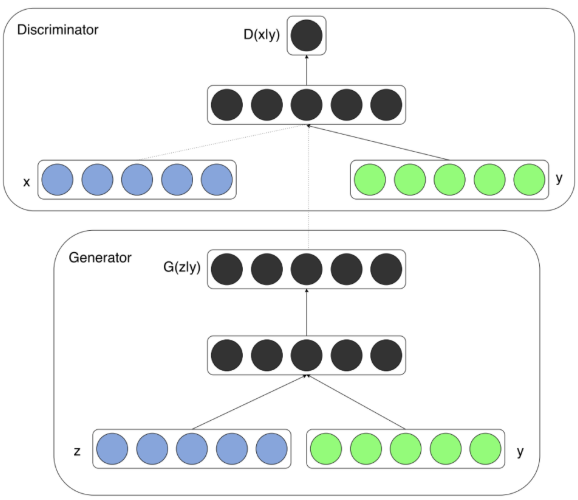
\includegraphics[width=4cm]{figures/1174039/chapter9/teori2.PNG}
            	\centering
           	\caption{Age-cGAN}
       	 \end{figure}

        \item Jelaskan dengan ilustrasi gambar sendiri arsitektur encoder network dari AgecGAN.

Arsitektur encoder biasanya digunakan untuk memodelkan struktur manifold dan membalikkan encoder untuk memproses data.

	\begin{figure}[H]
		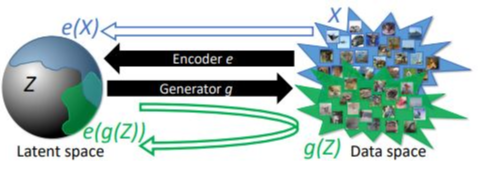
\includegraphics[width=4cm]{figures/1174039/chapter9/teori3.PNG}
            	\centering
           	\caption{Encoder Age cGANr}
       	 \end{figure}

        \item Jelaskan dengan ilustrasi gambar sendiri arsitektur generator network dari AgecGAN.

Arsitektur generator adalah sebuah array yang digunakan secara random, yang disebut seed. dari data seed tersebut, generator akan merubahnya menjadi sebuah gambar yang ukuran 28 x 28 dengan menggunakan Convolutional Neural Network.

	\begin{figure}[H]
		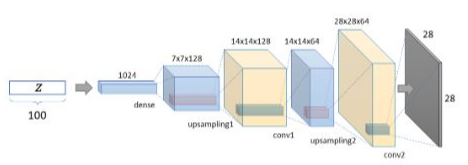
\includegraphics[width=4cm]{figures/1174039/chapter9/teori4.PNG}
            	\centering
           	\caption{Network Age cGAN}
       	 \end{figure}


        \item Jelaskan dengan ilustrasi gambar sendiri arsitektur discriminator network dari Age-cGAN.

Arsitektur diskriminator adalah CNN yang dapat menerima input gambar yang berukuran 28,28 serta menghasilkan angka biner yang menyatakan apakah data yang diinputkan merupakan dataset asli atau gambar dataset palsu.

	\begin{figure}[H]
		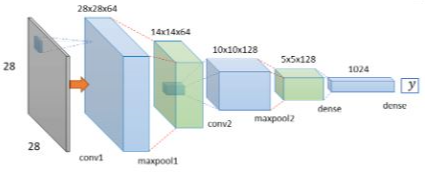
\includegraphics[width=4cm]{figures/1174039/chapter9/teori5.PNG}
            	\centering
           	\caption{Discriminator Age cGAN}
       	 \end{figure}


        \item Jelaskan dengan ilustrasi gambar apa itu pretrained Inception-ResNet-2 Model.

Pre-Trained Network atau Transfer Learning merupakan suatu metode penyelesaian yang memanfaatkan model yang sudah dilatih terhadap suatu dataset untuk menyelesaikan masalah dengan cara menggunakan sebagai starting point, memodifikasi dan mengupdate parameternya, sehingga sesuai dengan dataset yang baru.

	\begin{figure}[H]
		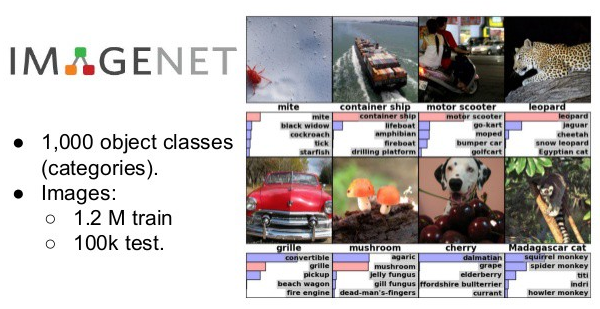
\includegraphics[width=4cm]{figures/1174039/chapter9/teori6.PNG}
            	\centering
           	\caption{Pretrained Inception ResNet}
       	 \end{figure}

        \item Jelaskan dengan ilustrasi gambar sendiri arsitektur Face recognition network Age-cGAN.

Face Recognition merupakan salah satu sistem yang mengimplementasi Deep Learning yang dapat mengenali wajah secara fisik dari gambar digital atau video frame.

	\begin{figure}[H]
		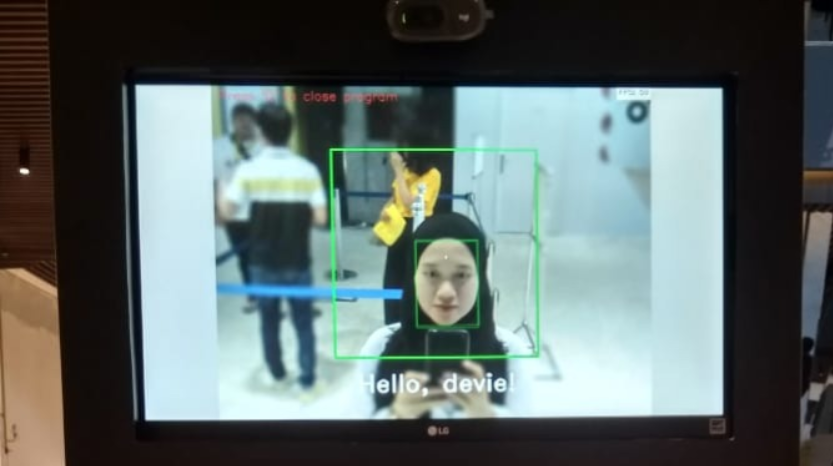
\includegraphics[width=4cm]{figures/1174039/chapter9/teori7.PNG}
            	\centering
           	 \caption{Face recognition network Age-cGAN}
       	 \end{figure}

        \item Sebutkan dan jelaskan serta di sertai contoh-contoh tahapan dari Age-cGAN.

Pada dari Age-cGan ni terdapat 2 tahapan dengan generator dan diskriminator. dimana untuk tahap generator sendiri membutuhkan vektor laten 100 serta menghasilkan gambar yang realistis dari dimensinya. sedangkan tahap diskriminator itu tahapan dimana memprediksi gambar yang diberikan nyata atau palsu.

	\begin{figure}[H]
		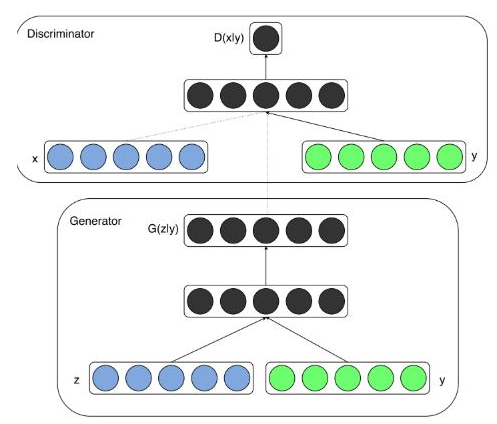
\includegraphics[width=4cm]{figures/1174039/chapter9/teori8.PNG}
            	\centering
           	 \caption{Tahap Age cGAN}
       	 \end{figure}

        \item Berikan contoh perhitungan fungsi training objektif.

Objektif Trainning ialah untuk meminimalkan loss function sebagai log likelihood function yang diberikan pada persamaan dimana D melambangkan trainning data.

	\begin{figure}[H]
		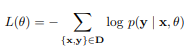
\includegraphics[width=4cm]{figures/1174039/chapter9/teori9.PNG}
            	\centering
           	 \caption{Training Objektif}
       	 \end{figure}

        \item Berikan contoh dengan ilustrasi penjelasan dari Initial latent vector approximation.

Latent vector approdimation kemampuan untuk membuat gamar yang realistis dan tajam serta menghasilkan gambar wajah pada usia target.

	\begin{figure}[H]
		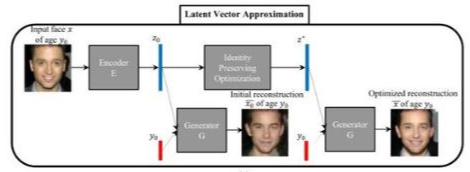
\includegraphics[width=4cm]{figures/1174039/chapter9/teori10.PNG}
            	\centering
           	 \caption{Initial Latent Vector Approximation}
       	 \end{figure}

        \item Berikan contoh perhitungan latent vector optimization.

Perhitungan lantent optimization menggunakan metode yang relatif sederhana, tergantung pada jumlah kecil parameter yang diperlukan, sehingga pada latent optimization dapat memetakan setiap gambar x dari dataset ke vektor acak dimensi rendah zi dalam ruang laten z.

	\begin{figure}[H]
		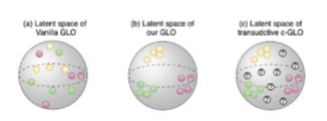
\includegraphics[width=4cm]{figures/1174039/chapter9/teori11.PNG}
            	\centering
           	 \caption{Latent Vector Optimization}
       	 \end{figure}

\begin{itemize}
\end{enumerate}

\subsection{Praktek}
\begin{enumerate}
\begin{itemize}

	\item Jelaskan bagaimana cara ekstrak file dataset Age-cGAN menggunakan google colab.
Menggunakan Google Colab, dimana membuat notebooks baru, kemudian membuat ekstraksi file dari link dataset.

		\lstinputlisting[firstline=1, lastline=4]{src/1174039/chapter9/chapter9.py}

	\item Jelaskan bagaimana kode program bekerja untuk melakukan load terhadap dataset yang sudah di ekstrak, termasuk bagaimana penjelasan kode program perhitungan usia.
Dibawah ini merupakan code untuk melakukan fungsi perhitungan usia.

		\lstinputlisting[firstline=6, lastline=31]{src/1174039/chapter9/chapter9.py}

	\item Jelaskan bagaimana kode program The Encoder Network bekerja dijelaskan dengan bahawa awam dengan ilustrasi sederhana.
Proses Encoder berfungsi untuk mempelajari pemetaan terbalik dari gambar wajah dan kondisi usia dengan vector latent Z.

		\lstinputlisting[firstline=33, lastline=73]{src/1174039/chapter9/chapter9.py}

	\itemJelaskan bagaimana kode program The Generator Network bekerja dijelaskan dengan bahawa awam dengan ilustrasi sederhana.
Proses Generator agar bekerja dengan baik dibutuhkan representasi dari gambar wajah dan vector kondisi sebagai inputan yang menghasilkan sebuah gambar.

		\lstinputlisting[firstline=75, lastline=104]{src/1174039/chapter9/chapter9.py}

        	\item Jelaskan bagaimana kode program The Discriminator Network bekerja dijelaskan dengan bahawa awam dengan ilustrasi sederhana.
Proses Discriminator untuk membedakan antara gambar asli dan gambar palsu.

		\lstinputlisting[firstline=116, lastline=148]{src/1174039/chapter9/chapter9.py}

        	\item Jelaskan bagaimana kode program Training cGAN bekerja dijelaskan dengan bahawa awam dengan ilustrasi sederhana.
Proses Training cGAN ini dengan load file .mat pada dataset lalu epoch sebanuak 500 kali.

		\lstinputlisting[firstline=150, lastline=167]{src/1174039/chapter9/chapter9.py}

        	\item Jelaskan bagaimana kode program Initial dan latent vector approximation bekerja dijelaskan dengan bahawa awam dengan ilustrasi sederhana.
Initial dan Latent Vector Approximation bekerja melakukan predicsi epoch yang telah di buat sebanyak 500 kali, dan nanti hasilnya ada di folder result.

		\lstinputlisting[firstline=169, lastline=217]{src/1174039/chapter9/chapter9.py}


\end{itemize}
\end{enumerate}

\subsection{Penanganan Error}
\begin{enumerate}
\begin{itemize}

\end{itemize}
\end{enumerate}

\subsection{Bukti Tidak Plagiat}
\begin{figure}[H]
\centering
	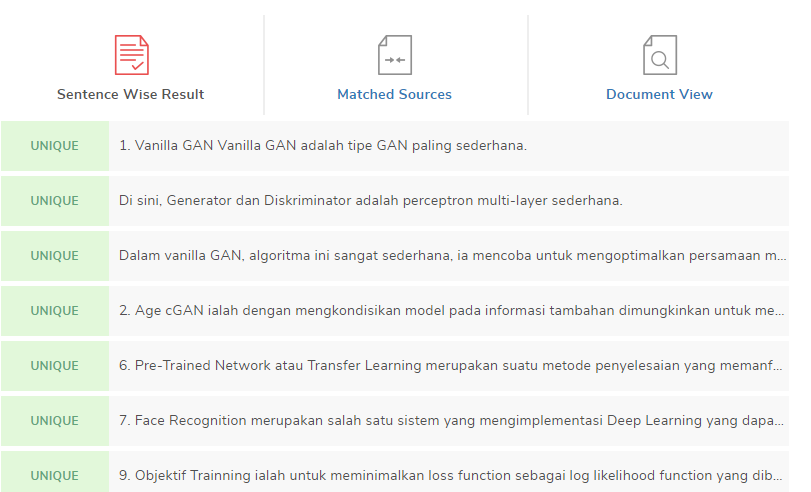
\includegraphics[width=4cm]{figures/1174039/chapter9/bukticekplagiarismechapter9.PNG}
	\caption{Bukti Tidak Melakukan Plagiat Chapter 9}
\end{figure}